\documentclass[border=10pt]{standalone}
\usepackage{pgfplots}
\pgfplotsset{compat=1.18}
\begin{document}
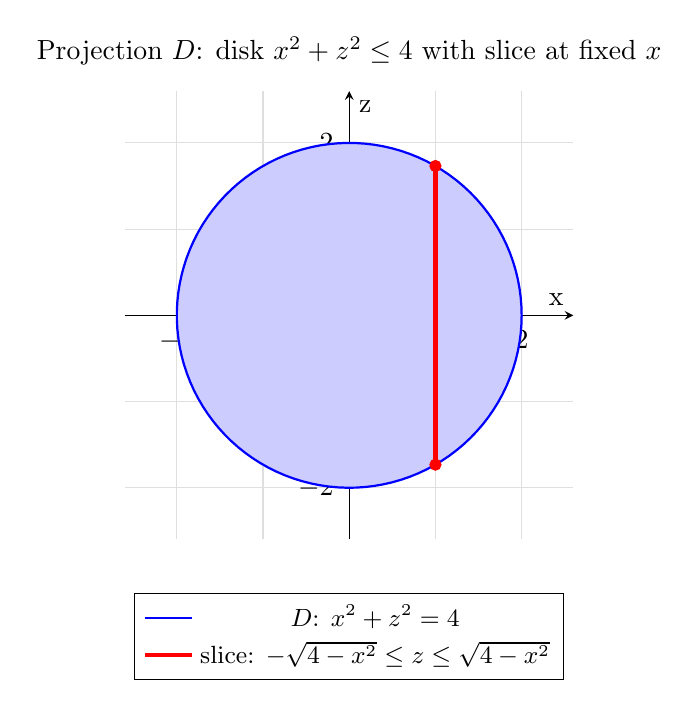
\begin{tikzpicture}
\begin{axis}[
    axis lines=middle,
    xlabel={x}, ylabel={z},
    xmin=-2.6, xmax=2.6, ymin=-2.6, ymax=2.6,
    title={Projection $D$: disk $x^2+z^2\le 4$ with slice at fixed $x$},
    axis equal image,
    grid=both,
    grid style={gray!25},
    legend style={at={(0.5,-0.12)}, anchor=north, legend columns=1, font=\small}
]
\addplot[blue, thick, fill=blue!20, domain=0:360, samples=120] ({2*cos(x)}, {2*sin(x)}) \closedcycle;
\addlegendentry{$D$: $x^2+z^2=4$}
\addplot[red, ultra thick] coordinates {(1, {-1.7320508}) (1, {1.7320508})};
\addlegendentry{slice: $-\sqrt{4-x^2}\le z\le\sqrt{4-x^2}$}
\addplot[only marks, mark=*, red] coordinates {(1, {-1.7320508}) (1, {1.7320508})};
\end{axis}
\end{tikzpicture}
\end{document}